\label{sec:approx}

In this section, we present the main novel contribution of our paper
for approximating XADDs within a fixed error bound.  Since the point
of XADD approximation is to shrink its size, we refer to our method of
approximation as XADD Compression (\textsc{XADDComp}).

Following previous work on ADD compression~\cite{apricodd}, we note
that decision diagrams should be compressed from the bottom up ---
merging leaves causes simplifications to ripple upwards through a
decision diagram removing vacuous decisions and shrinking the decision
diagram.  For example, after merging leaves in
Figure~\ref{fig:stepfunfig}(a), we note that the only remaining
decision in \ref{fig:stepfunfig}(b) is $x < 3$.  Hence, we focus on a
leaf merging approach to \texttt{XADDComp}, which poses two questions:
(1) what leaves do we merge, and (2) how do we find the best
approximation of merged leaves?  We answer these two questions in the
following subsections.

%A novel method for approximating piecewise linear functions with
%bounded error. The goal of this algorithm is to reduce the number of
%partitions of a piecewise linear function represented in case
%form. This represents the ability to automatically identify and remove
%locally unimportant constraints, whose removal results in a small
%change in the represented function in exchange for a significant
%improvement in the efficiency of computations with these
%functions. XADDs already permit compactness by exploring variable and
%context independencies, so our approximate approach goes further to
%merge partitions as a form of removing dependencies that had little
%influence in the represented function.

%%%%%%%%%%%%%%%%%%%%%%%%%%%%%%%%%%%%%%%%%%%%%%%%%%%%%%%%%%%%%%%%%%%%%%
%% I am glad that you have improved so many things, but it does seem
%% bad that there were so many "mistakes".
%%
%% Not mistakes per se, but just too much technical detail that
%% detracted from the main storyline that defines the paper.
%% What you were writing was more for the style of a journal article 
%% or thesis, so its appropriate when you go to write those.
%%
%% Also you should work on writing very succinct sentences.  Typically
%% a lot of what you're writing can be expressed in much less space, or 
%% does not really need to be explained, or does not need to be explained
%% in the place you are explaining it.
%%%%%%%%%%%%%%%%%%%%%%%%%%%%%%%%%%%%%%%%%%%%%%%%%%%%%%%%%%%%%%%%%%%%%%


%%%%%%%%%%%%%%%%%%%%%%%%%%%%%%%%%%%%%%%%%%%%%%%%%%%%%%%%%%%%%%%%%%%%%%
%%
%% TODO: need to show accumulated error in merges
%% TODO: need to indicate with under-bracket, which nodes are being merged.
%%
\begin{figure}[t!]
\centering
  \subfigure[Original] {
  	\begin{minipage}{.25\textwidth}
	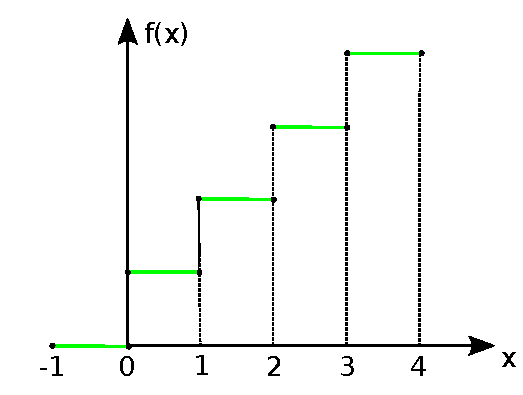
\includegraphics[width=\textwidth]{Figures/stepfun/succ1.pdf}
	\end{minipage}
	\begin{minipage}{.2\textwidth}
	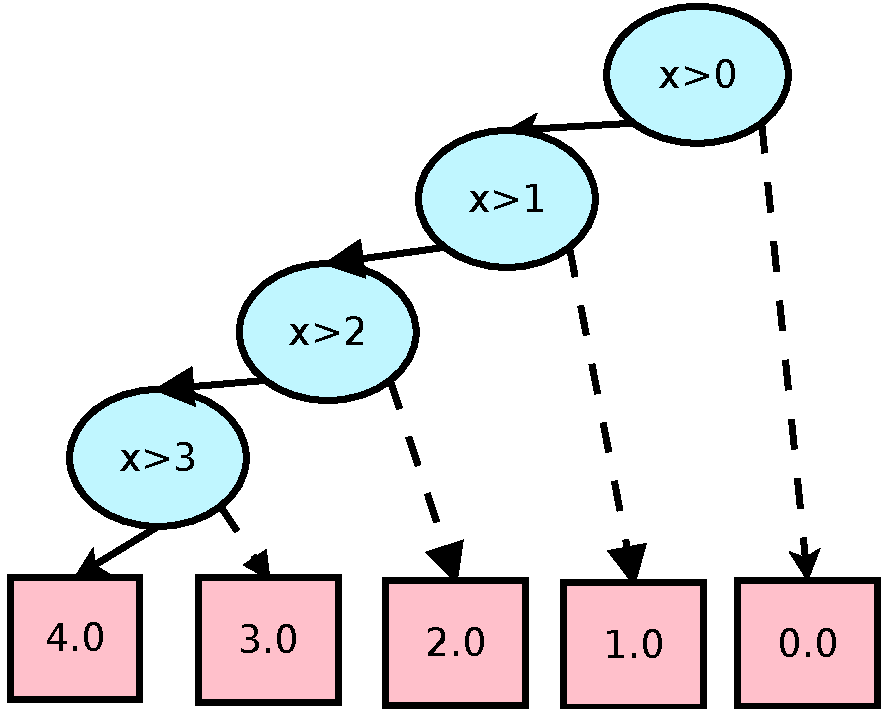
\includegraphics[width=\textwidth]{Figures/xadds/succ1xadd.pdf}
	\end{minipage}
	\label{original}
  }
\subfigure[Step1] {
  	\begin{minipage}{.25\textwidth}
	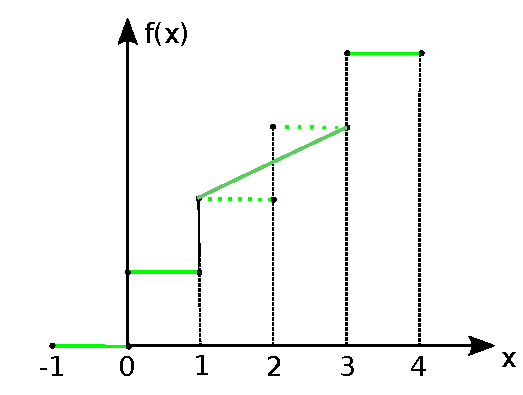
\includegraphics[width=\textwidth]{Figures/stepfun/succ2.pdf}
	\end{minipage}
	\begin{minipage}{.2\textwidth}
	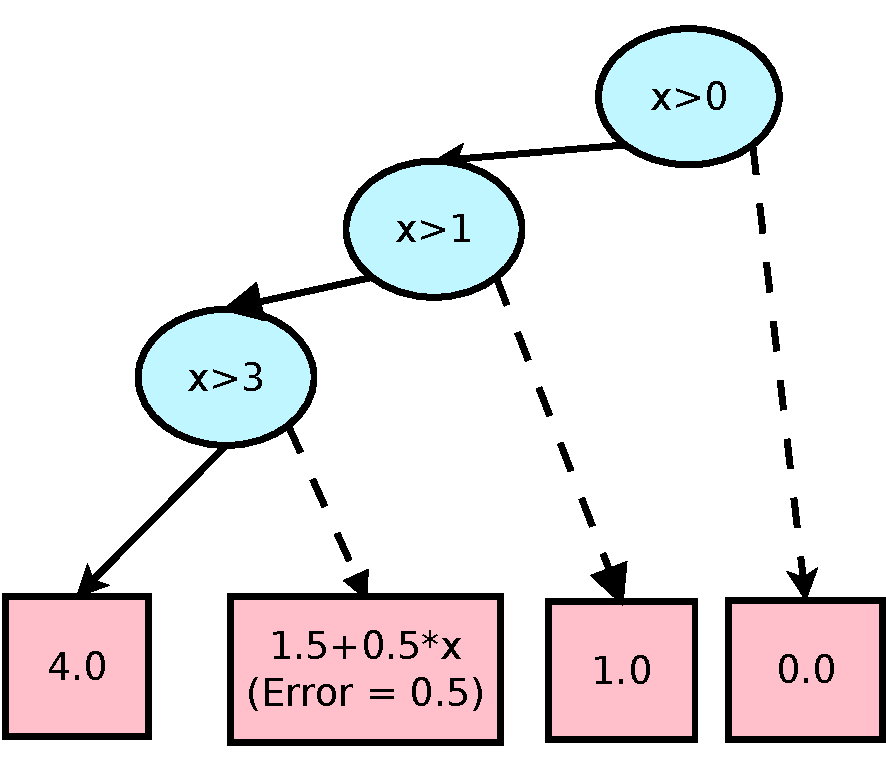
\includegraphics[width=\textwidth]{Figures/xadds/succ2xadd.pdf}
	\end{minipage}
	\label{step1} 
}
\subfigure[Step2]{
  	\begin{minipage}{.25\textwidth}
	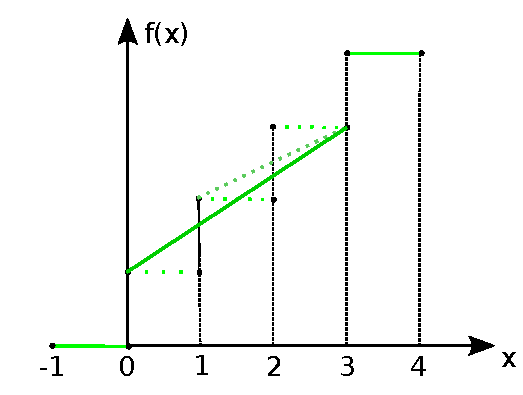
\includegraphics[width=\textwidth]{Figures/stepfun/succ3.pdf}
	\end{minipage}
	\begin{minipage}{.2\textwidth}
	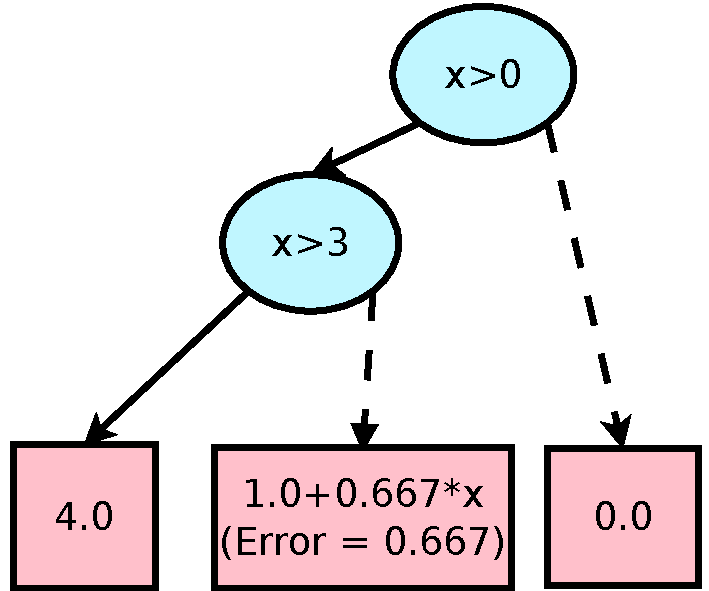
\includegraphics[width=\textwidth]{Figures/xadds/succ3xadd.pdf}
	\end{minipage}
	 \label{step2}
}
\caption{ \footnotesize Successive pair merging XADD compression for a simple 1D example.
At each step two nodes are chosen for merging, the best approximating
hyperplane is determined according to Section~\ref{sec:leaf_approx},
and if the accumulated error is within required bounds, the leaves are
merged and internal XADD structure simplified to remove unneeded
decisions.}  \label{fig:steplining}
\end{figure}
%%%%%%%%%%%%%%%%%%%%%%%%%%%%%%%%%%%%%%%%%%%%%%%%%%%%%%%%%%%%%%%%%%%%%%

\subsection{Successive Leaf Merging}

%% See notes below on pseudocode... there will be too many questions
%% about undefined notation and there are too many details to fix
%% before the deadline.  I don't think you need anything more than
%% the simple diagrammatic explanation of Successive Leaf Merging,
%% as long as you denote the error accumulation.

Since it would be combinatorially prohibitive to examine all possible
leaf merges in an XADD, our approximation algorithm in
Algorithm~\ref{alg:approx} uses a systematic search strategy of successive
pairwise merging of leaves. The idea is simple and is illustrated
in Figure~\ref{fig:steplining}. The bounded error property is
guaranteed by accumulating the amount of error "used" in every merged
leaf and avoiding any merges that exceed a maximum error threshold $\epsilon$.
However, we have not yet defined how to find the lowest error approximation
of a pair of leaves in \texttt{PairLeafApprox}, which we provide next.

%%%%%%%%%%%%%%%%%%%%%%%%%%%%%%%%%%%%%%%%%%%%%%%%%%%%%%%%%%%%%%%%%%%%%%
%%
\incmargin{1.5em}
\linesnumbered
\begin{algorithm}[t!]
\dontprintsemicolon
%% NOTE: $error$ is read as e*r*r*o*r... you want $\mathit{error}$
%% NOTE: Follow notation that is used in the paper, always L for a leaf/partition.
%% NOTE: All algorithm notation has to be consistent, later algorithms
%%       don't use this \KwIn, \KwOut and use := in place of \gets.
%\KwIn{A piecewise linear function $V$, relative\_allow\_error}
%\KwOut{Approximated version of $V$.}
%% NOTE: Relative error adds numerous explanation complications and
%%       I think it is hard to justify over the HMDP just passing in
%%       an allowed error bound which is how things are done in the 
%%       literature.  This is the cleanest way to do things and a 
%%       more complex approach should not be taken unless it is empirically
%%       better.
%%$allow\_error \gets M * relative\_allow\_error$
$\hat{\epsilon} \gets 0$ \emph{// The max amount of error used so far}\;
$\hat{X} \gets X$ \emph{// The approximated XADD}\;
$\Open := \{ L_i \} = \{ \l \phi_i, f_i \r \} \in \hat{X}$\emph{// cases in $\hat{X}$}\;
\While{$\Open \neq \emptyset$} {
	$L_1 := \Open.\mathit{pop}()$\;
	\For{$ L_2 \in \Open$}  { 
                \emph{// Merge and track accumulated error}\;
		$f^* := $\texttt{PairLeafApprox}$(L_1, L_2)$\emph{// Sec~\ref{sec:leaf_approx}}\;
%                \emph{// Track accumulated error in merge}\;
	        $f^*.\Error := f^*.\Error + $\\\hspace{18mm}$\max(f_1.\Error,f_2.\Error)$\;
                \emph{// Keep merge if within error bounds}\;
		\If {$f^*.\Error < \epsilon$}
		{       
                        $\hat{\epsilon} := \max(\hat{\epsilon}, f^*.\Error)$\;
			$\Open.\mathit{remove}(L_2)$\;
                        \emph{//Merge leaves and simplify $\hat{X}$}
			$\hat{X}.f_1 := f^*, \; \hat{X}.f_2 := f^*$\; 
                        % \texttt{Simplify($\hat{X}$)}\; $ Not defined, so omit
			\; 
			$\Open.\mathit{insert}(\l \phi_1 \lor \phi_2, f^* \r)$\;
		}
	}
}
\Return{$(\hat{X},\hat{\epsilon})$}\emph{// Comp. XADD and error used}\;
\caption{\footnotesize 
 \texttt{XADDComp}(XADD $X$, $\epsilon$) $\longrightarrow$ $(\hat{X},\hat{\epsilon})$}
\label{alg:approx}
\end{algorithm}
\decmargin{1.5em}
%%%%%%%%%%%%%%%%%%%%%%%%%%%%%%%%%%%%%%%%%%%%%%%%%%%%%%%%%%%%%%%%%%%%%%

\subsection{Pairwise Leaf Approximation}

\label{sec:leaf_approx}

%% Following is verbose and a lot of it obvious, or already explained,
%% or complicating matters in ways not required to get the key insights.
%%
%We now focus on the pairwise case linear function approximation. The
%most important step in our solution to piecewise linear function
%approximation is the iterative linear program based algorithm for
%obtaining optimal, that is, max-error minimizing, case linear function
%to approximate any pair of case linear functions. In order to explain
%our algorithm more conveniently, we make the following consideration.
%
%Since the continuous domain of a case linear function is independent
%of boolean variable decisions, they do not interfere with the
%constrained maximization of the linear functions and therefore don't
%affect the merging of case linear functions. Hence, for clarity, we
%will consider piecewise linear functions whose partitions are defined
%only with linear inequalities.
%
%We can now define the optimal merging of case linear functions as an
%optimization problem. 

%% Need to get to bilinear optimization problem by the end of the first
%% paragraph.
In pairwise leaf merging, we must address the following fundamental
problem: given two XADD leaves represented by their case partitions
$L_1 = \l f_1, \phi_1 \r$ and $L_2 = \l f_2, \phi_2 \r$, our goal is to
determine the best linear case approximation of $L_1$ and $L_2$.  As
it must represent $L_1$ and $L_2$, the solution must be defined in
both regions and is therefore of the form $L^* =
\l f^*,\phi_1 \lor \phi_2 \r$.  Since we restrict to linear XADDs, 
$f_1 = \vec{c_1}^T (\vec{x}^T,1)^T$, $f_2 = \vec{c_2}^T (\vec{x}^T,1)^T$ and 
$f^* = \vec{c^*}^T (\vec{x}^T,1)^T$ (assuming
$\vec{c_1},\vec{c_2},\vec{c^*} \in \mathbb{R}^{m+1}$ where $\vec{x} \in \mathbb{R}^{m}$).  
Hence the optimization problem reduces
to one of finding the optimal weight vector $\vec{c^*}$ satisfying the
following bilinear saddle point optimization problem:
\begin{equation} 
\min_{\vec{c}^*} \max_{i \in \{ 1, 2 \}} \max_{\vec{x} \in C(\phi_i)} \bigg| \underbrace{\vec{c_i}^T \mb \vec{x}\\1 \me}_{f_i} - \underbrace{\vec{c^*}^T \mb \vec{x}\\1 \me}_{f^*} \bigg| \label{eq:optimglo} 
\end{equation}
This is bilinear due to the inner product of $\vec{c^*}$ with $\vec{x}$.
%This is a saddle point optimization problem due to the
%$\min_{\vec{c}^*} \max_{\vec{x}}$ and bilinear due to the inner product
%of $\vec{c^*}$ with $\vec{x}$.
%
%In short, this says that we need to find the weight vector $\vec{c^*}$
%which \emph{minimizes the maximum absolute difference} between the hyperplanes defined
%by $f^*$ and $f_1, f_2$, but only for the valid
%$\vec{x}$ in the respective polytopes $C(\phi_1)$ and $C(\phi_2)$ where
%each leaf $f_1$ and $f_2$ is valid.

%%%%%%%%%%%%%%%%%%%%%%%%%%%%%%%%%%%%%%%%%%%%%%%%%%%%%%%%%%%%%%%%%%%%%%
\begin{figure}[t!]
\center
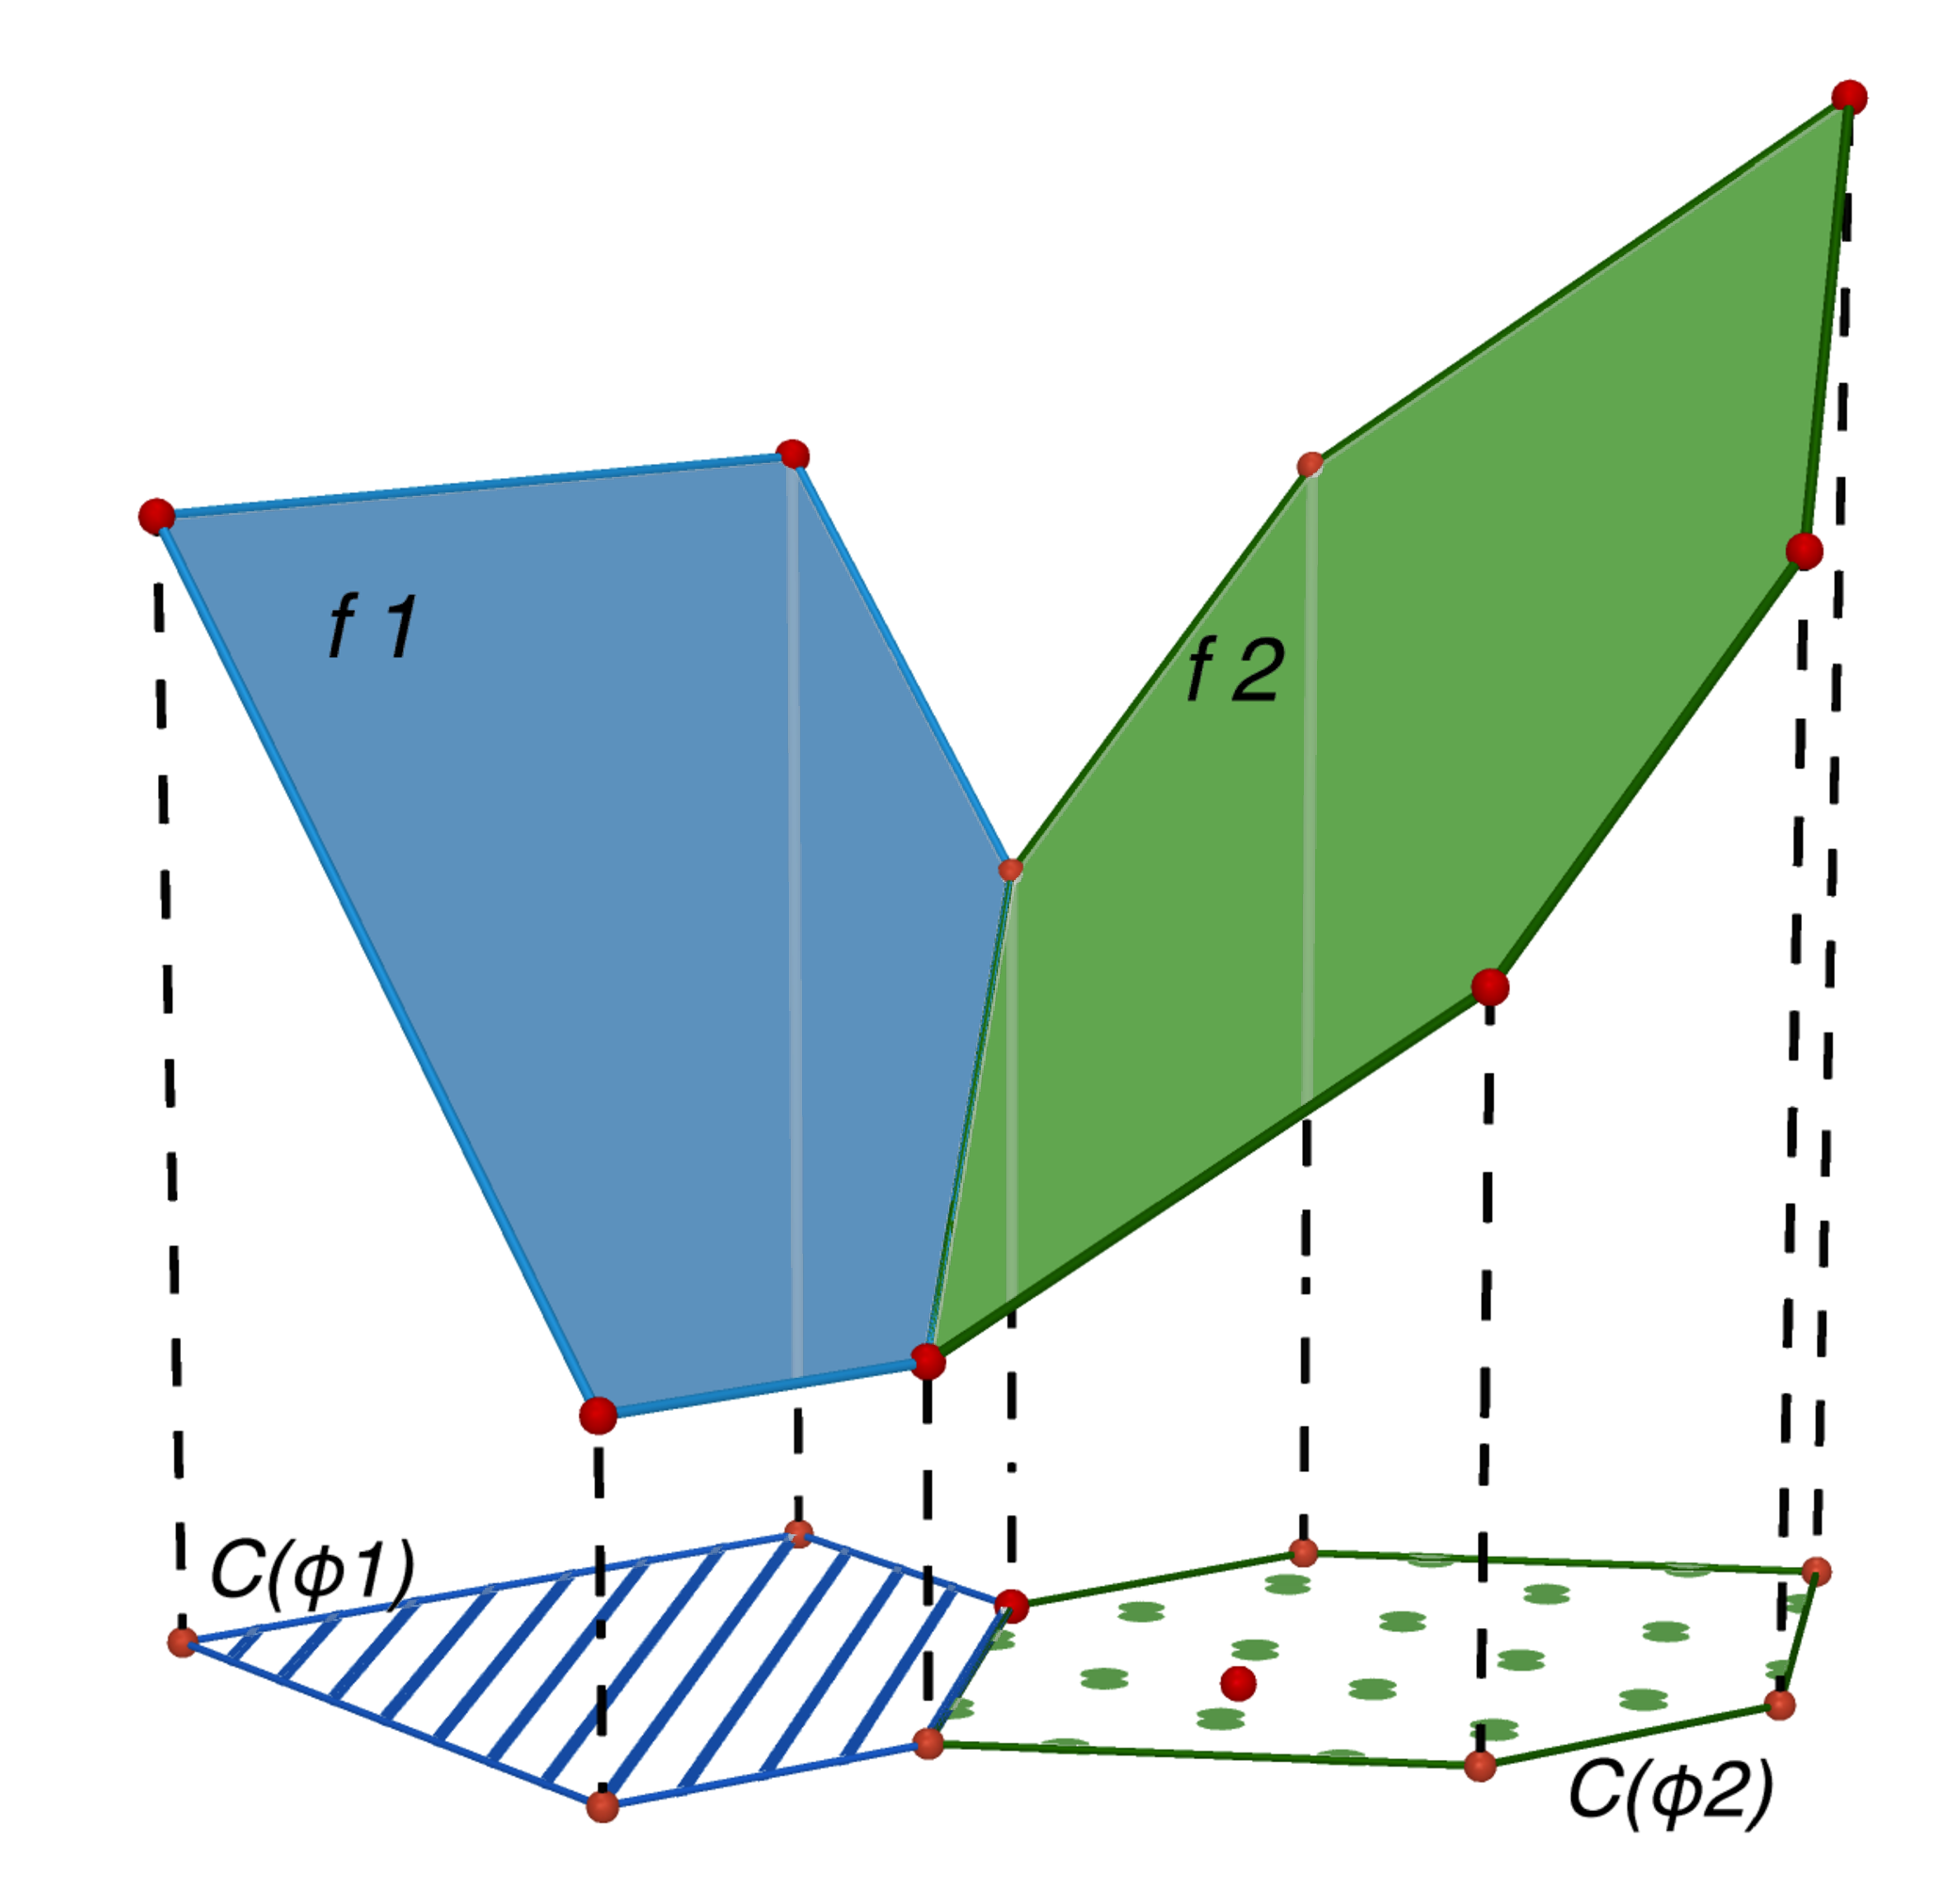
\includegraphics[trim = 2cm 0cm 2cm 0cm, height=0.25\textwidth,width=0.2\textwidth]{Figures/optimDiag/optdiagram1.pdf} 
\hspace{2mm}
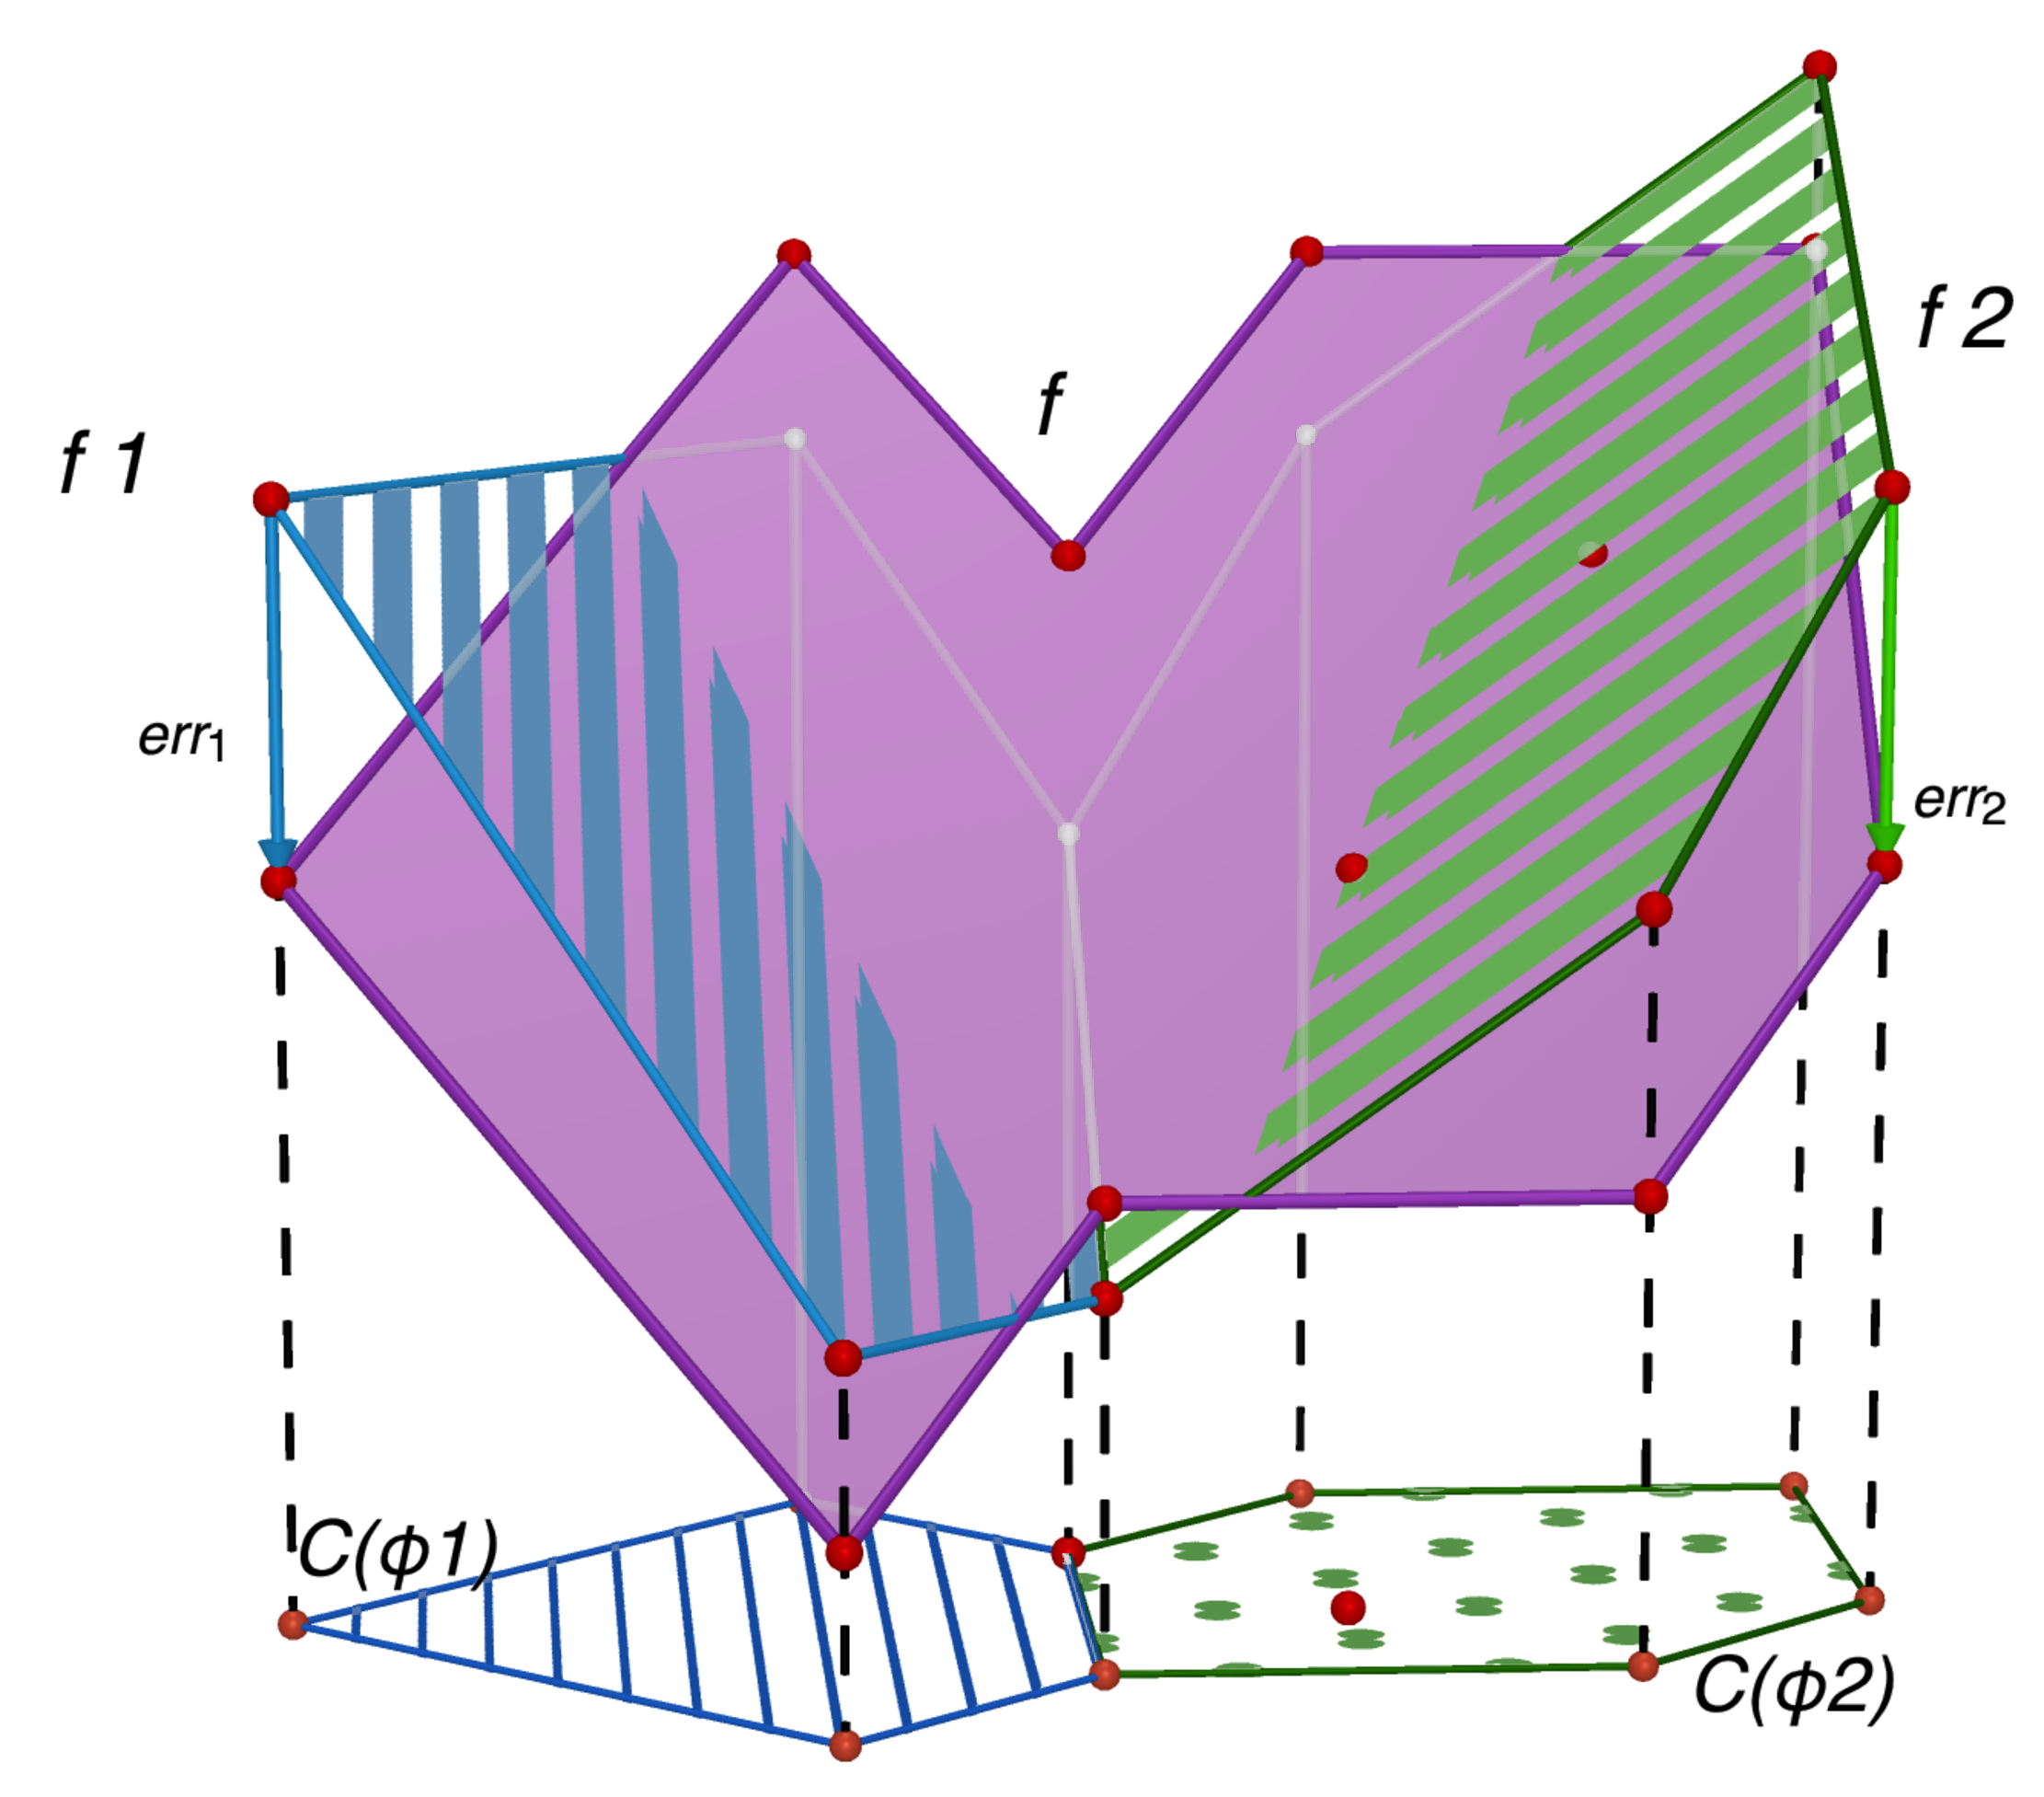
\includegraphics[trim = 2cm 0cm 2cm 0cm, height=0.25\textwidth,width=0.2\textwidth]{Figures/optimDiag/optdiagram2.pdf}
\caption{\footnotesize Illustration of the pairwise leaf approximation problem: \emph{(left)} the original linear leaf functions $f_1$ and $f_2$ in their respective (single) polytope regions $\phi_1$ and $\phi_2$; \emph{(right)} a linear approximation $f$ overlaid on $f_1$ and $f_2$ in their regions showing errors at the polytope vertices.}
\label{fig:optim} 
\end{figure}
%%%%%%%%%%%%%%%%%%%%%%%%%%%%%%%%%%%%%%%%%%%%%%%%%%%%%%%%%%%%%%%%%%%%%%

To better understand the structure of this bilinear saddle point
problem, we refer to Figure~\ref{fig:optim}, which shows on the
left, two functions $f_1$ and $f_2$ and the respective single polytope
regions $C(\phi_1)$ and $C(\phi_2)$ where $f_1$ and $f_2$ are
respectively valid.  On the right, we show a proposed approximating
hyperplane $f$ within the regions $C(\phi_1)$ and $C(\phi_2)$.
Clearly we want to choose the $f^*=f$ that minimizes the absolute
difference between $f$ and $f_1,f_2$ within their respective polytopes.
On account of this perspective and recalling that $C(\phi_i)
= \bigcup_j \PT(\theta_{ij})$, we can rewrite~\eqref{eq:optimglo} as
the following bi-level linear optimization problem:\footnote{
To obtain a true bi-level \emph{linear} program, we need \emph{two} separate
second stage constraints to encode that $\epsilon$ is larger than each
side of the absolute value (the argument of the absolute value and its
negation), but this is a straightforward absolute value expansion in a
linear program that we will consider implicit to avoid notational clutter.}
\begin{align}
\min_{\vec{c}^*,\epsilon} \; & \epsilon \label{eq:bilevel} \\
s.t. \;       & \epsilon \geq \left( \!\!
  \begin{array}{ll}
  \max\limits_{\vec{x}} \! & \left| \vec{c_i}^T \! \mb \vec{x}\\1 \me \! - \vec{c^*}^T \! \mb \vec{x}\\1 \me \right| \\ 
  s.t. \;              \! & \vec{x} \in \PT(\theta_{ij})
  \end{array} \!\!\! \right); \forall i \in \{ 1,\!2 \}, \forall \theta_{ij} \nonumber
\end{align}
While it may seem we have made little progress with this rewrite
of~\eqref{eq:optimglo} --- this still appears to be a difficult
optimization problem, we can make an important insight that allows
us to remove the second stage of optimization altogether.  While
implicitly it appears that the second stage would correspond to an
infinite number of constraints --- one for each
$\vec{x} \in \PT(\theta_{ij})$, we return to Figure~\ref{fig:optim}.
Since each of $f$, $f_1$, and $f_2$ are all linear and
$C(\phi_1),C(\phi_2)$ represent (unions of) linear convex polytopes,
we know that the \emph{maximum difference} between $f$ and $f_1,f_2$ must
occur at the \emph{vertices} of the respective polytope regions.
Thus, denoting $\vec{x_{ij}^k}$ ($k = \{ 1 \ldots N_{ij} \}$) as a vertex of
the linear convex polytope defined by $\theta_{ij}$, we can obtain a
\emph{linear program} version of~\eqref{eq:optimglo} with a \emph{finite} 
number of constraints:
\begin{align}
\min_{\vec{c}^*,\epsilon} \; & \epsilon \label{eq:linear_exp} \\
s.t. \;       & \epsilon \geq \left| \vec{c_i}^T \! \mb \vec{x_{ij}^k}\\1 \me \! - \vec{c^*}^T \! \mb \vec{x_{ij}^k}\\1 \me \right|; 
\begin{array}{l}
\forall i \in \{ 1,\!2 \}, \forall \theta_{ij} \nonumber,\\ 
\forall k \in \{ 1 \ldots N_{ij} \}
\end{array}
\end{align}
Unfortunately, the drawback of this single linear programming approach
is that for $n_{ij}$ linear constraints in $\PT(\theta_{ij})$, the
number of vertices of the polytope may be exponential, i.e., $N_{ij} =
O(\exp n_{ij})$.  

However, we make one final critical insight: while we may have
an exponential number of constraints in~\eqref{eq:linear_exp}, we have
a very efficient way to evaluate for a \emph{fixed} solution $\vec{c}^*$,
what single point $\vec{x_{ij}^k}$ in each polytope $\PT(\theta_{ij})$
provides the maximum error --- this is exactly what the second stage
linear program in~\eqref{eq:bilevel} provides.  Hence, this suggests a
very efficient constraint generation approach to
solving~\eqref{eq:linear_exp}:

\vspace{1mm}
\noindent \texttt{PairwiseLeafApprox}($L_1,L_2$) $\longrightarrow$ ($\vec{c}^*,\epsilon$):
\vspace{-2mm}
\begin{enumerate}
\item Initialize $\vec{c}^*$ to an arbitrary value and the constraint set $C$
to be empty, i.e., $C = \emptyset$.
\item Given $\vec{c}^*$, for each $i \in \{ 1,2\}$ and for each $\theta_{ij}$, generate the $\vec{x_{ij}^k}$ s.t.
\begin{align*}
\vec{x_{ij}^k} := \argmax_{\vec{x}} \! & \left| \vec{c_i}^T \! \mb \vec{x}\\1 \me \! - \vec{c^*}^T \! \mb \vec{x}\\1 \me \right| \\ 
  s.t. \;              \! & \vec{x} \in \PT(\theta_{ij})
\end{align*}
and add the following pair of constraints to $C$:
\begin{align*}
  C := C \; \cup \; & \{ \epsilon > \vec{c_i}^T ({\vec{x_{ij}^k}}^T,1)^T - \vec{c^*}^T ({\vec{x_{ij}^k}}^T,1)^T \} \\
         \; \cup \; & \{ \epsilon > \vec{c^*}^T ({\vec{x_{ij}^k}}^T,1)^T - \vec{c_i}^T ({\vec{x_{ij}^k}}^T,1)^T \}
%  C := C \; \cup \; & \{ \epsilon > \vec{c_i}^T \! \mb \vec{x_{ij}^k} \\1 \me \! - \vec{c^*}^T \! \mb \vec{x_{ij}^k}\\1 \me \} \\
%         \; \cup \; & \{ \epsilon > \vec{c^*}^T \! \mb \vec{x_{ij}^k}\\1 \me - \vec{c_i}^T \! \mb \vec{x_{ij}^k} \\1 \me \}
\end{align*}
encoding that $\epsilon$ must be greater than the absolute error induced
by $f_i - f^*$ at the vertex point $\vec{x_{ij}^k}$.  
%This is an important constraint to
%add because it corresponds to the $\vec{x_{ij}^k}$ with the maximum error.
\item Solve the LP of~\eqref{eq:linear_exp} w.r.t. the subset of constraints in $C$ to obtain a new $\vec{c}^*_{\mathit{new}}$.
\item If $\vec{c}^* = \vec{c}^*_{\mathit{new}}$, return the optimal solution $\vec{c}^*$ and its error $\epsilon$, otherwise go to step 2.
\end{enumerate}
Once the last step returns $\vec{c}^*,\epsilon$, we have the best $f^*$ and corresponding
maximum error $\epsilon$ given leaves $L_1$ and $L_2$, thus performing the optimal pairwise
leaf approximation problem that we set out to address.


{\bf TODO: Scott left off here... need to refine above explanation... consider putting content into a formal algorithm, continue to theoretical guarantees.}

Terminates at convergence in finite steps.


{\bf Theorem} {\it Algorithm~\ref{alg:glo} always terminates and produces the optimal solution for the optimization described in Eqs.~\ref{eq:minc},~\ref{eq:errcij},~\ref{eq:polymax}.} 

To prove the optimality of the solution obtained, we observe that at the beginning of the loop the algorithm always keeps an optimal approximation $f$ for all $points$ stored. Using this $f$ the $MAX\_ERROR$ routine computes new points that are the maximum error points for this $f$. If there are new points, these are added to the stored points and $BEST\_APPROX$ computes a new $f$ that minimizes in all stored points. As we return to the start of the loop we have a new optimal approximation. If there are no new points, this means that the current $f$ minimizes the error in the points that maximize its error therefore it minimizes the maximal error in all regions and is the optimal solution.  As the algorithm only terminates when there are no new points, and in this case the solution is optimal, if the algorithm terminates, its solution is optimal.
 Next we prove that the algorithm must terminate: First, the formulae $\phi$  are finite and define a finite number of polytopes. Second, for all polytopes defined, there is a finite number of inequalities and correspondingly a finite number of vertices. At each non terminal iteration at least one new polytope vertex must be added to the stored $points$ list, as there are finitely many vertices, the number of iterations must be finite, so the algorithm terminates.


In practice, terminates with much fewer than exponential number of constraints.

This defines the algorithm \textsc{PairwiseCaseMax} called in line X of Algorithm~\ref{alg:approx}.

%% Formal pseudocode in the form of algorithms has to be completely
%% an unambiguously specified -- every function call has to be defined
%% in another algorithm or equation, every structured argument or
%% has to be formally defined.  I've removed the existing pseudocode
%% because the above is more than adequate to understand the pairwise
%% merge and it will take a lot of editing to achieve the formal
%% level of quality needed in the existing pseudocode at much greater
%% length than the above description.  We're going to run out of space
%% as is and I don't think the pseudocode makes an further 
%% contribution to the above description.
%%
%% Some notes: 
%% - what are Remap and ApplyRemap?  these really get into details of implementation
%%   that are not crucial for understanding the key insights of the algorithm
%% - the range of all variables has to be defined (point, sol+, obj+, etc)
%% - function calls should not be in a math font, they should be textsc or texttt
%% - function calls have to be formally defined in other algorithms or equations
%% - max_points.add(sol+,sol-) is not clear, should use set notation: 
%%      max_points := max_points \cup {sol+} \cup {sol-}
%% - NEG_INF is -\infty in Latex
%% - Poly has not been defined in the text, previously Polyt had been defined
%% - It is taking three columns of a lot of (undefined) notation to describe
%%   the list enumerated algorithm above
%%
%% The AAAI-12 SDP pseudocode should obey the above properties, if not, it is
%% a mistake and should be fixed in the upcoming HMDP discussion.






